\documentclass[10pt,conference,compsocconf]{IEEEtran}

% create a shortcut to typeset table headings
\newcommand\tabhead[1]{\small\textbf{#1}}

%\usepackage{times}
%\usepackage{balance}
\usepackage{url}
\usepackage{graphicx}	% For figure environment
\usepackage{graphicx}
\usepackage{caption}
\usepackage{subcaption}

\begin{document}
\title{Natural Feature Detection for Augmented Reality}

\author{
  Benjamin Flueck, Hongyi Liu\\
  Department of Computer Science, ETH Zurich, Switzerland\\
}

\maketitle

\begin{abstract}
The Abstract goes here
\end{abstract}

\section{Introduction}

With the proliferation of powerful mobile phones and their cameras augmented reality (AR) application are now on the verge on becoming ubiquitous. While AR applications existed for along time and can be ported to mobile platforms, many of them rely on predefined patterns. While this is perfectly fine research purposes in a lab it is a considerable inconvenience for every day applications. The goal of this project is therefore to implement a simple augmented reality application that explores the possibility of using arbitrary patterns while considering the limitations of mobile phones.

\section{Method}

Our Application uses a simple combination of a feature detection \& extraction schema supplemented by a KLT tracker. In a first step the application acquires an initial image which should be sufficiently textured. We then do a feature extraction on this image as a starting point for the KLT tracking. As the KLT tracker is limited to  tracking feature points from one frame to the next it is only suitable for tracking already known feature points and not for recovery or detection of the target object. We therefore supply the application with a simple re-detection procedure. This is done by taking a frame and proceeding with a feature detection on it. The features are then directly matched with the ones from the initial image. While the KLT tracker is faster than a full feature detection, extraction, and matching cycle it is prone to loosing track of features and drifting over time. Our application therefore interlaces the KLT tracking with regular re-detection cycles when either the quality or the number of the tracked features drop below certain thresholds. In the end this results in a fast and never the less robust tracking of the initial image.

\subsection{Feature Selection and Matching}
In order to be used for our approach the features for the tracking and re-detection have to full-fill certain criteria. They have to be rotation and preferably be scaling invariant and they must be fast to compute. While the rotational invariance is a must the scaling invariant can be substituted with computing the same features on different scales on the image. Due to the relatively small number of features we are operating on, the matching of those features can be computed with a straight forward brute force approach as this takes an insignificant time compared to the feature detection and extraction. \\
In this sense, we need to investigate different types of feature detection and feature extraction methods. We have compared the following features for their computational effort and quality of matches they yield; ORB, Briskd, Fast, Star, Good, Dense\\
We conduct two experiment as below:

\subsubsection{First experiment, Run time evaluation}

For this part of the study, we have an experimental setup that runs on an Android-capable phone system. We will evaluate the time consumption for feature detection (detect step) and feature description (compute step). We will load five different images from storage, and for each image, we will run the descriptor five times, creating 25 set of data for each feature detector/descriptor. The final results were the average of data points. Here we try to use all feature detectors that can run on android.\\
Result: (feature detector)\\

\begin{table}[!ht]
  \centering
  \begin{tabular}{|c|c|c|c|c|c|c|}
    \hline
     & Orb&Briskd&Fast&Star&good&dense\\
    \hline
    Time(second)&0.511&0.481&0.122&4.224&1.547&\textgreater5 \\
    \hline
  \end{tabular}
  \caption{different feature detection method time consumption compare.}
\end{table}
 
Result: (feature descriptor)\\

\begin{table}[!ht]
  \centering
  \begin{tabular}{|c|c|c|c|}
    \hline
     & Orb&Briskd&Brief\\
    \hline
    Time(second)&0.812&0.122&0.162 \\
    \hline
  \end{tabular}
  \caption{different feature extraction method time consumption compare.}
\end{table}

From this part, we learned that method star, good, dense are way too slow for our approach.\\

\subsubsection{Second experiment, performance evaluation}

Here we will analysis three different type of feature detectors in this section, respecitively: orb, briskd, and fast, and three different kinds of descriptors: orb, briskd, and brief. We sought to work with various combinations of detectors and descriptors on one pair of images, and display the result on the image pair. \\



\begin{table}[!ht]
  \centering
  \begin{tabular}{|c|c|c|c|c|}
    \hline
    \tabhead{Det-des}&
    \multicolumn{1}{|p{0.15\columnwidth}|}{\centering\tabhead{Keypoints from pic1}} &
    \multicolumn{1}{|p{0.15\columnwidth}|}{\centering\tabhead{Keypoints from pic2}}&
    \multicolumn{1}{|p{0.15\columnwidth}|}{\centering\tabhead{Matches number}}&
    \multicolumn{1}{|p{0.1\columnwidth}|}{\centering\tabhead{Inlier ratio}} \\
    \hline
    Orb-orb & 500 & 500 & 326 & 56\%\\
    \hline
    Orb-briskd & 499 & 498 & 324 & 60\%\\
    \hline
    Orb-brief & 500 & 500 & 244 &	55\%\\
    \hline
    Briskd-orb &	902 &	1164 &	598 &	21\%\\
    \hline
    Briskd-briskd &	903 &	1164 &	600 &	22\%\\
    \hline
    Briskd-brief &	902 &	1164 &	591 &	29\%\\
    \hline
    Fast-orb &	1428 &	2305 &	1209 &	43\%\\
    \hline
    Fast-briskd &	1433 &	2305	 &1109 &	45\%\\
    \hline
    Fast-brief &	1428 &	2305 &	1210 &	45\%\\
    \hline
  \end{tabular}
  \caption{Perform evaluation of different feature detector and extractor.}
  \label{tab:table1}
\end{table}

Illustrated below is the result picture we have obtained through the course of the experiment: within which, red circle corresponds to the keypoint found by the detector, green circles(smaller) represents matches, while blue circles(even smaller) correspond to inlier detected by findhomograph function.\\


\begin{figure}[!ht]
        \centering
        \begin{subfigure}[b]{0.15\textwidth}
                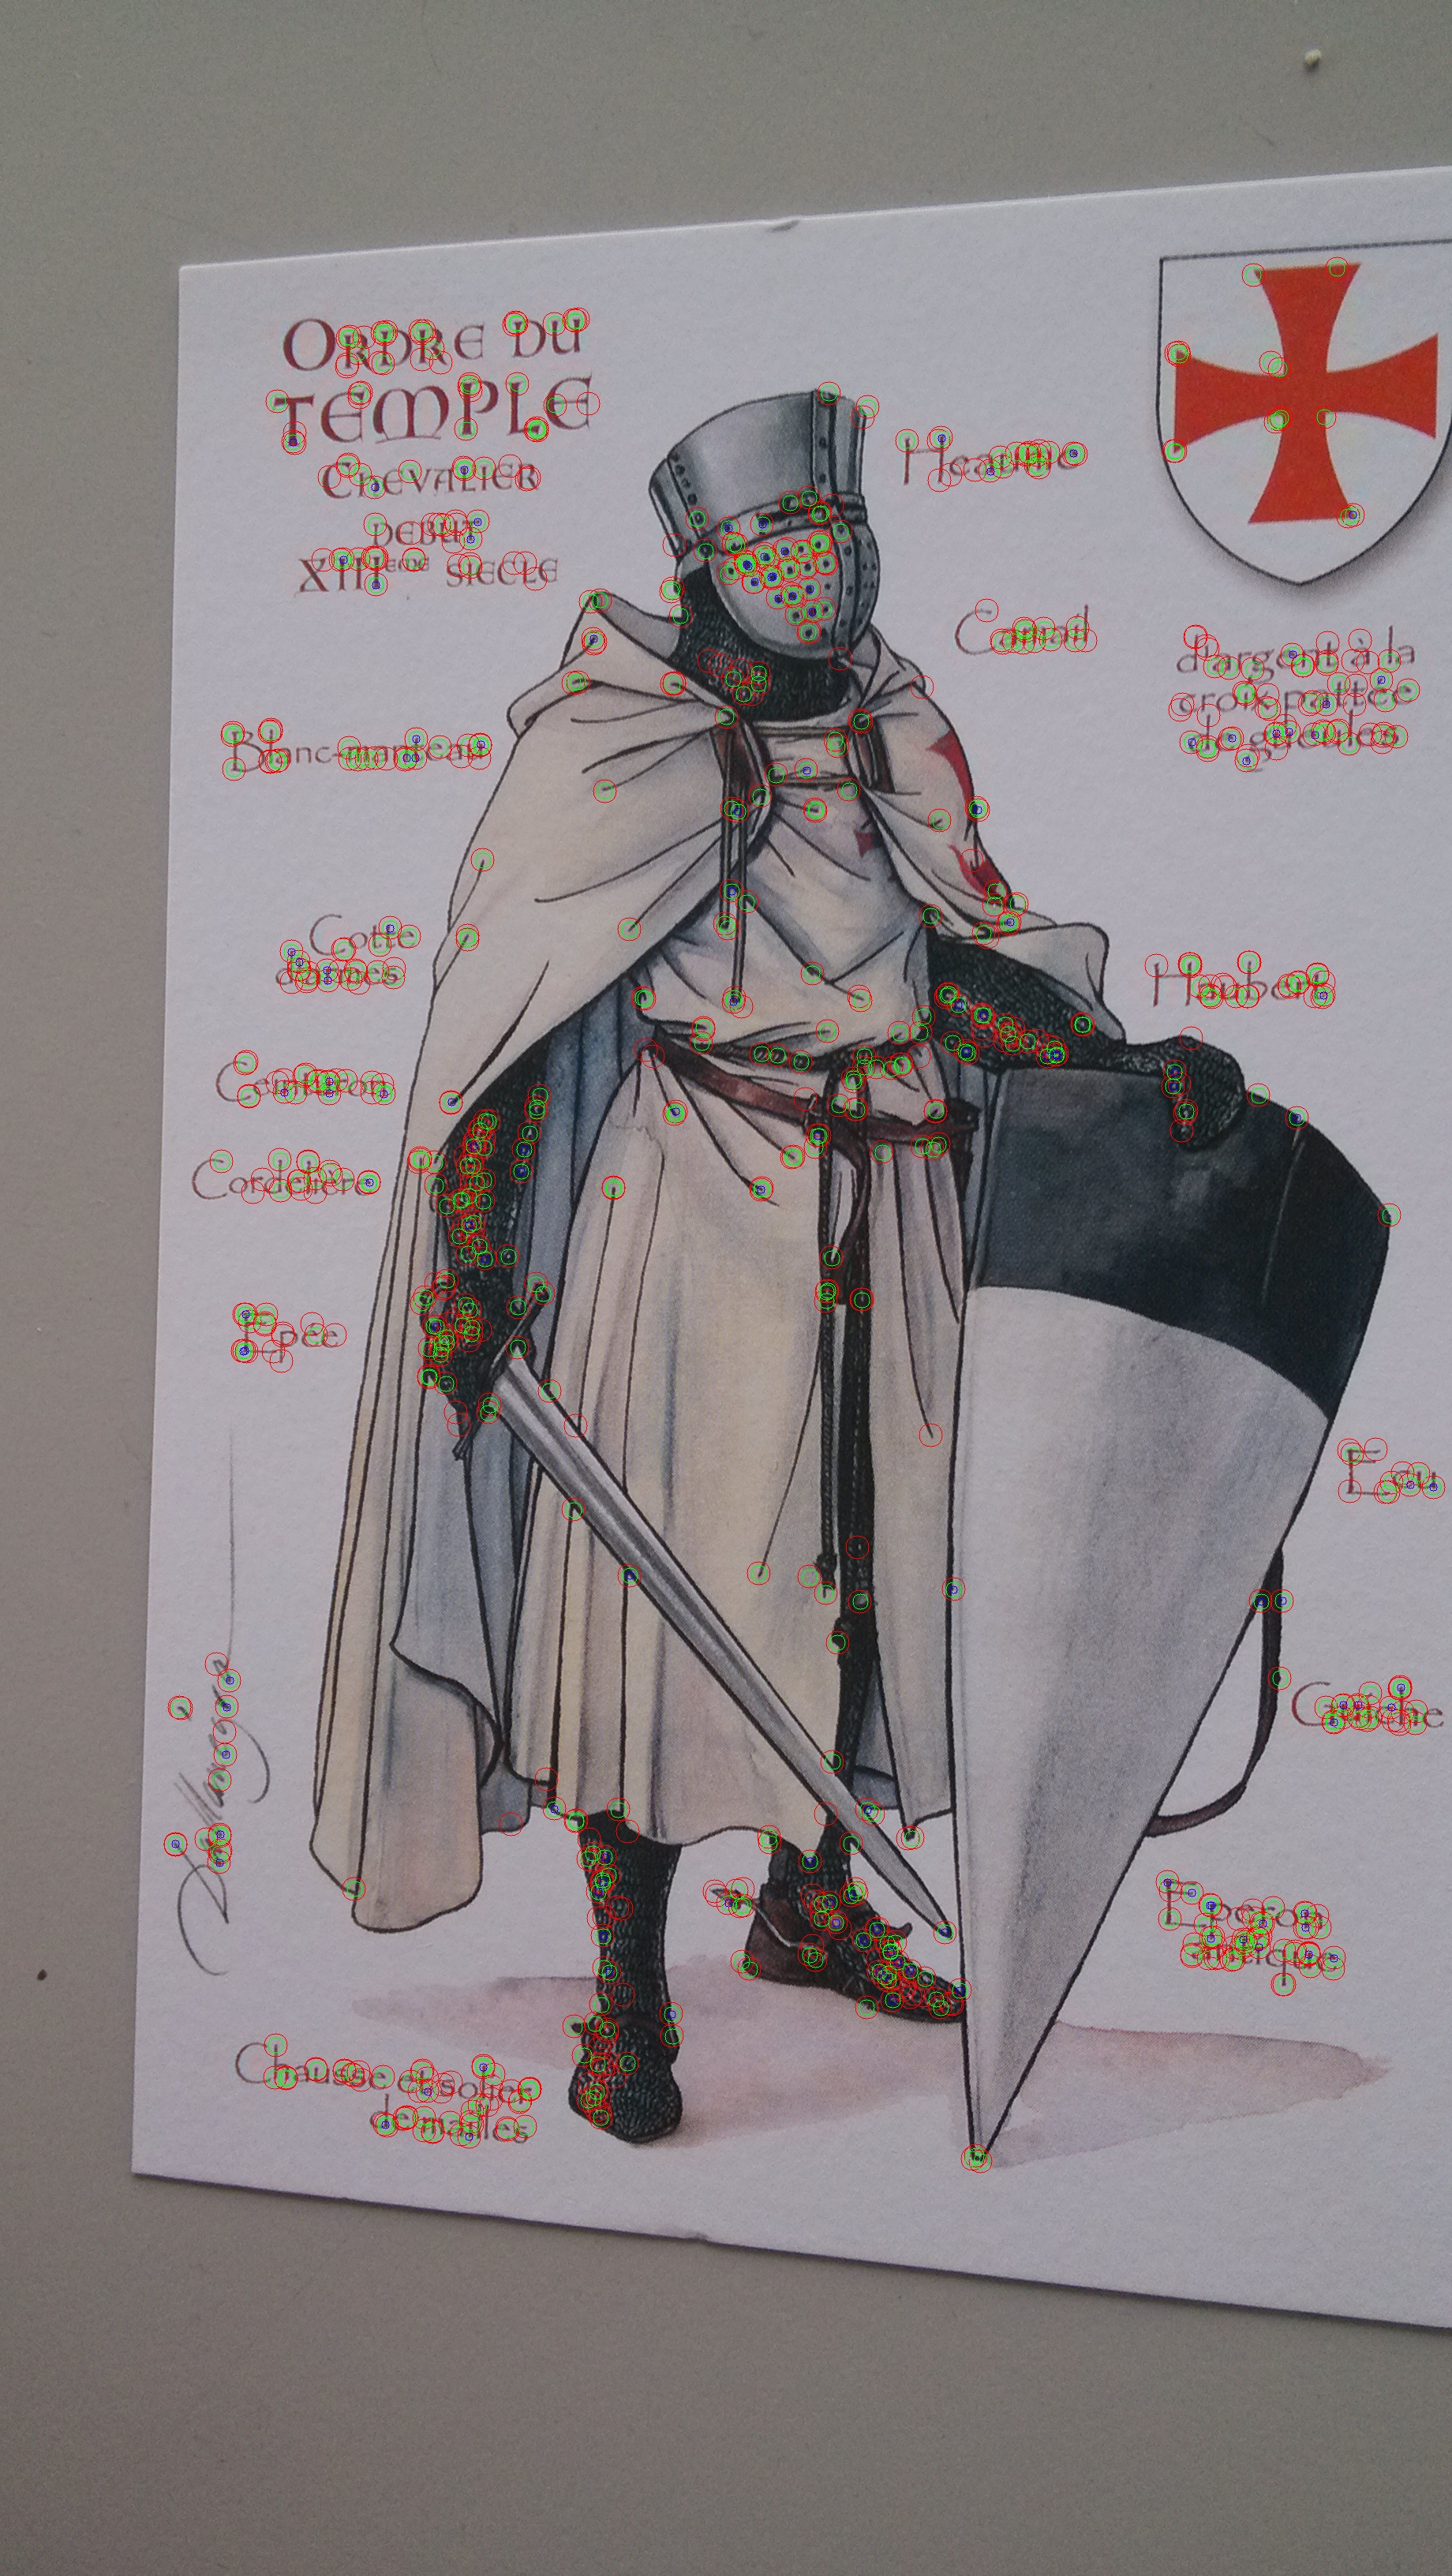
\includegraphics[width=\textwidth]{b}
                \caption{briskd-briskd}
                \label{fig:b}
        \end{subfigure}%
        ~ %add desired spacing between images, e. g. ~, \quad, \qquad etc.
          %(or a blank line to force the subfigure onto a new line)
        \begin{subfigure}[b]{0.15\textwidth}
                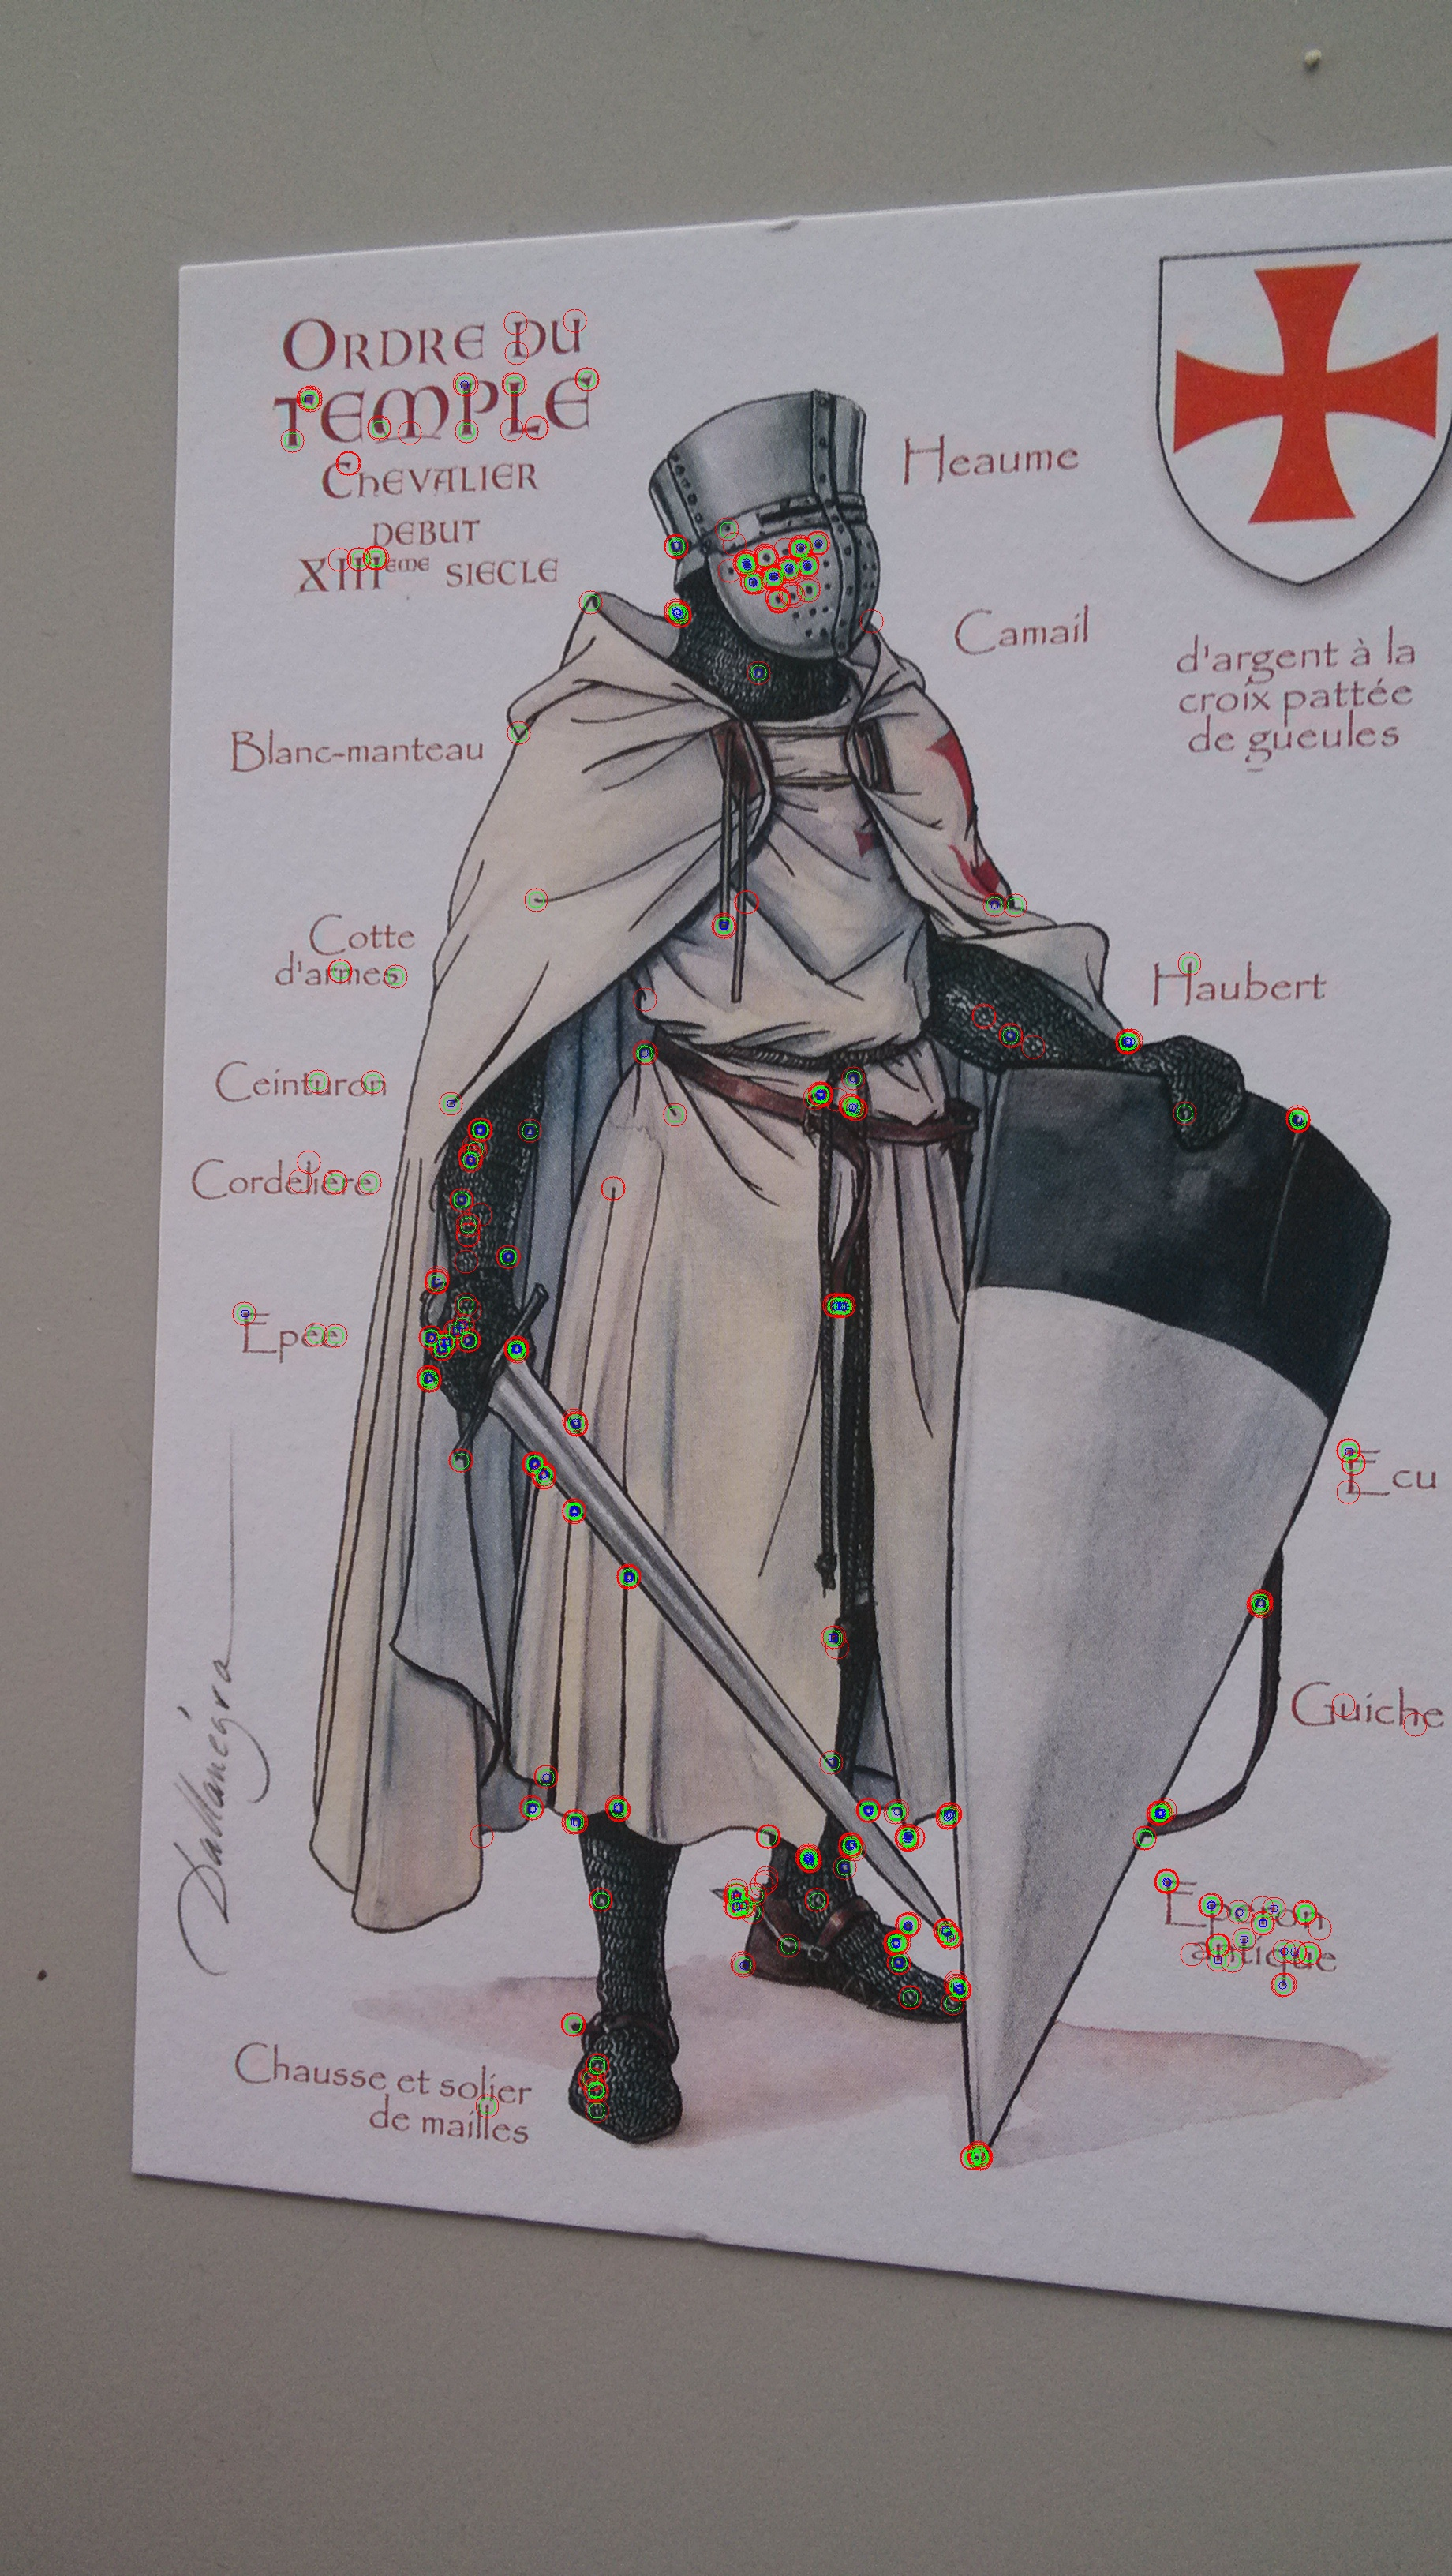
\includegraphics[width=\textwidth]{o}
                \caption{Orb-orb}
                \label{fig:o}
        \end{subfigure}
        ~ %add desired spacing between images, e. g. ~, \quad, \qquad etc.
          %(or a blank line to force the subfigure onto a new line)
        \begin{subfigure}[b]{0.15\textwidth}
                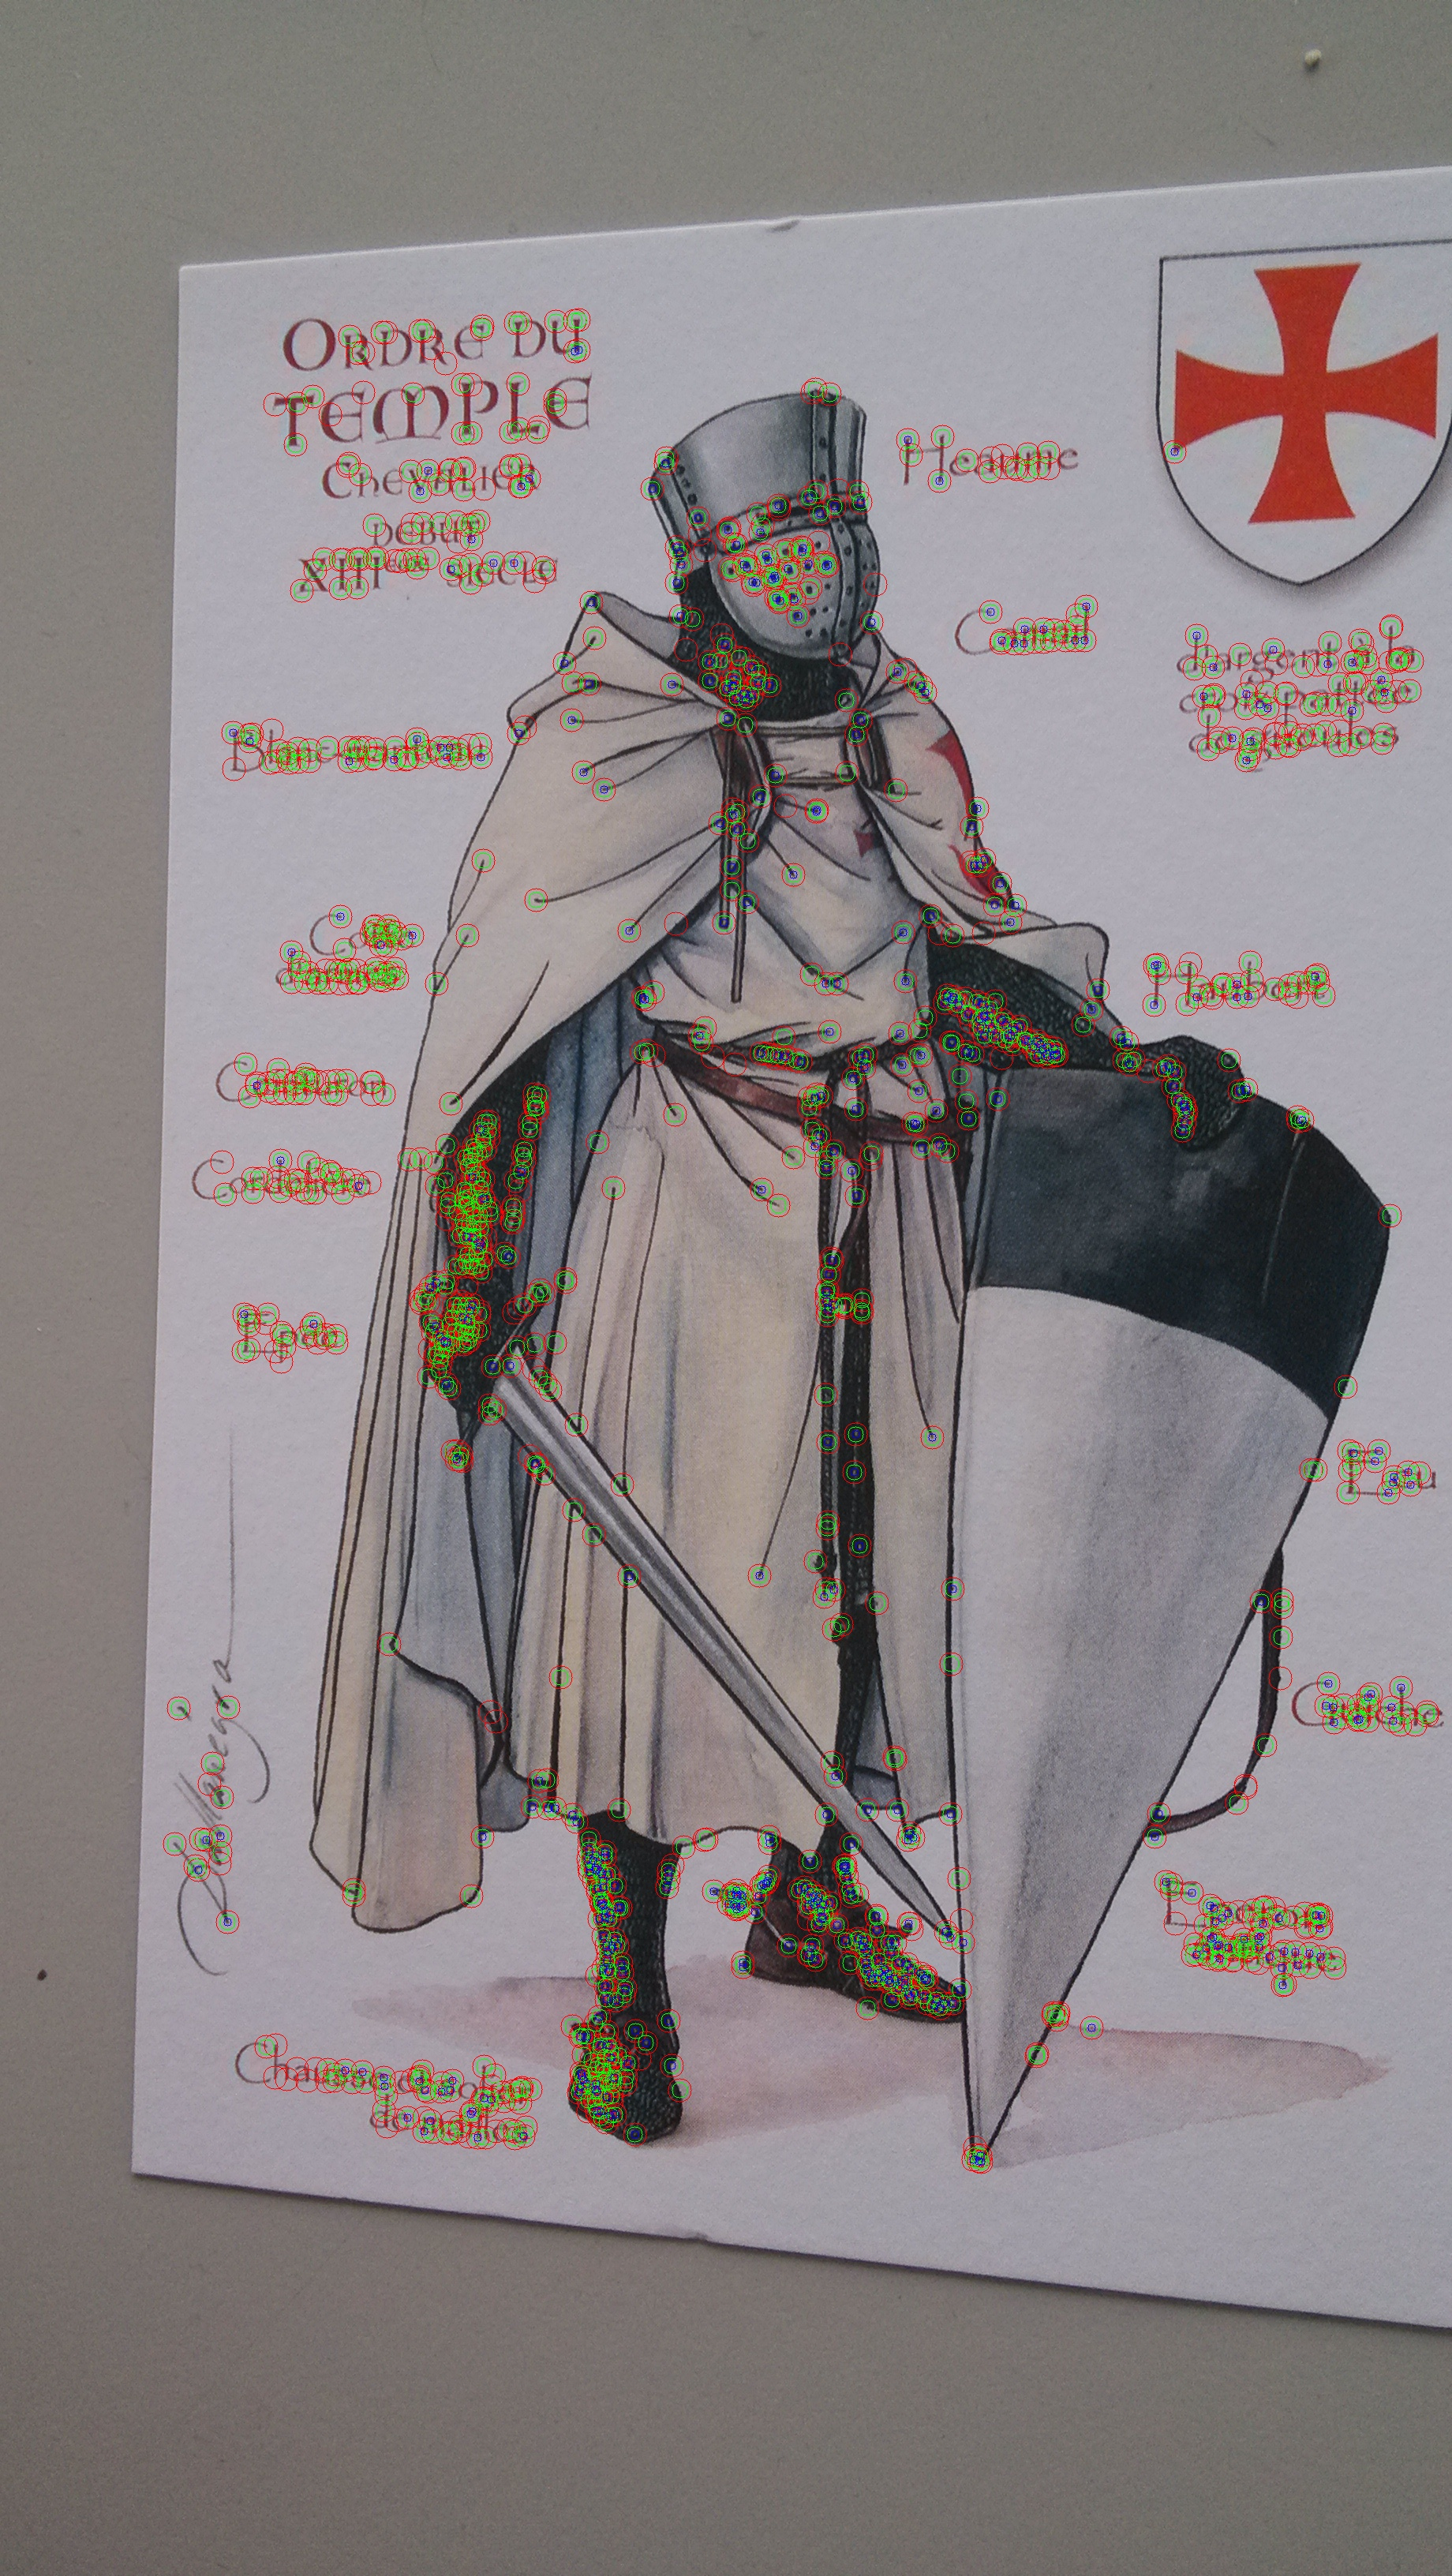
\includegraphics[width=\textwidth]{f}
                \caption{Fast-brief}
                \label{fig:f}
        \end{subfigure}
        \caption{keypoints, matches, inliner result of different detectors and extractors}\label{fig:animals}
\end{figure}

We can clearly observe the differences of keypoints, matches, inlier points selected by different feature detectors.\\

From the experiment above, we observe a correspondence between percentage of inlier ratio and the detector type, as a consequent, the detector and extractor ORB shall be our choice in later application.\\

\subsection{Motion blur and solution}

When we start camera, and move it, the blur effect will occur. The motion blur problem might cause by default setting of camera itself. It have a significant effect on our application. When ever motion blur appear, our estimate homo-graph will fail and frame rate will went low. To investigate what is the actual cause of low frame rate and homo-graph problem, we conduct an experiment.\\

In this experiment, we will load 8 different image pairs into our setup, and get parameters from them.
Five image pairs are normal, clear image. Three of them are different blurred images pairs(normal+blur and blur+blur). Then we will investigate the time consumption of keypoint detection, extraction, matching, homograph finding. The keypoints detected in both images will also be counted, as well as the matching number set up by brute force approach will be illustrated, at last, the inlier ratio computed by homograph will be considered.\\

This is the result:\\

\begin{table}[!ht]
  \centering
  \begin{tabular}{|c|c|c|c|c|c|c|c|c|}
    \hline
    \tabhead{ }&
    \multicolumn{1}{|p{0.05\columnwidth}|}{\centering\tabhead{detect time}} &
    \multicolumn{1}{|p{0.05\columnwidth}|}{\centering\tabhead{compute time}}&
    \multicolumn{1}{|p{0.05\columnwidth}|}{\centering\tabhead{match time}}&
    \multicolumn{1}{|p{0.05\columnwidth}|}{\centering\tabhead{find homo time}}&
    \multicolumn{1}{|p{0.05\columnwidth}|}{\centering\tabhead{KP 1}}&
    \multicolumn{1}{|p{0.05\columnwidth}|}{\centering\tabhead{KP 2}}&
    \multicolumn{1}{|p{0.05\columnwidth}|}{\centering\tabhead{match number}}&
    \multicolumn{1}{|p{0.05\columnwidth}|}{\centering\tabhead{inlier ratio}} \\
    \hline
    N1&	69.2ms&	74.6ms&	9.8ms&	8.4ms&	250&	250&	161&	67\%\\
    \hline
    N2&	48.6ms&	73.4ms&	3.2ms&	14.3ms&	250&	250&	153&	52\%\\
    \hline
    N3&	52.7ms&	66.8ms&	3.4ms&	9.3ms&	250&	250&	149&	51\%\\
    \hline
    N4&	56.4ms&	72.7ms&	1.9ms&	16.7ms&	250&	250&	154&	43\%\\
    \hline
    N5&	68.7ms&	87.0ms&	3.2ms&	7.9ms&	250&	250&	169&	53\%\\
    \hline
    N-b1&	36.2ms&	76.7ms&	5.5ms&	228.4ms&	246&	250&	128&	10\%\\
    \hline
    N-b2&	44.9ms&	70.6ms&	2.7ms&	256.9ms&	250&	250&	94&	7\%\\
    \hline
    B-b&	60.9ms&	109.3ms&	3.3ms&	258.9ms&	250&	246&	72&	9\%\\
    \hline
  \end{tabular}
  \caption{N1-5 means normal image pairs, N-b means normal image and blurred image, B-b means blurred image pairs.}
  \label{tab:table1}
\end{table}

\begin{figure}[!ht]
        \centering
        \begin{subfigure}[b]{0.2\textwidth}
                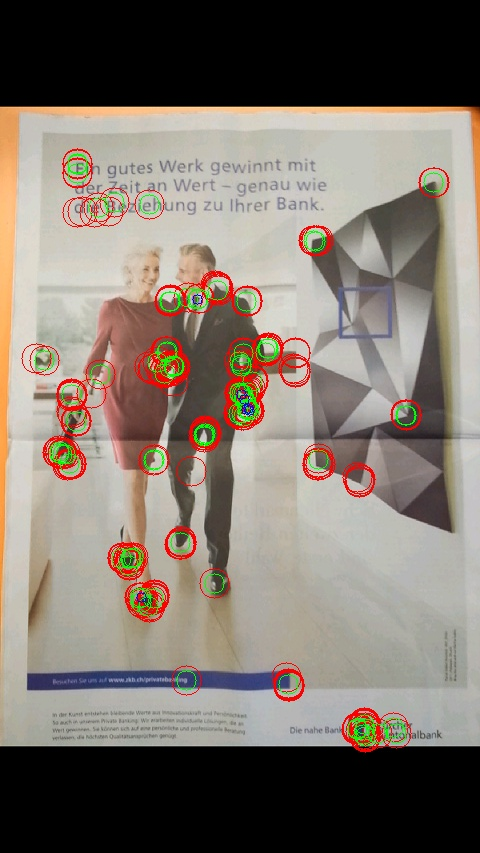
\includegraphics[width=\textwidth]{badly2}
                \caption{keypoint detected in normal image}
                \label{fig:badly2}
        \end{subfigure}%
        ~ %add desired spacing between images, e. g. ~, \quad, \qquad etc.
          %(or a blank line to force the subfigure onto a new line)
        \begin{subfigure}[b]{0.2\textwidth}
                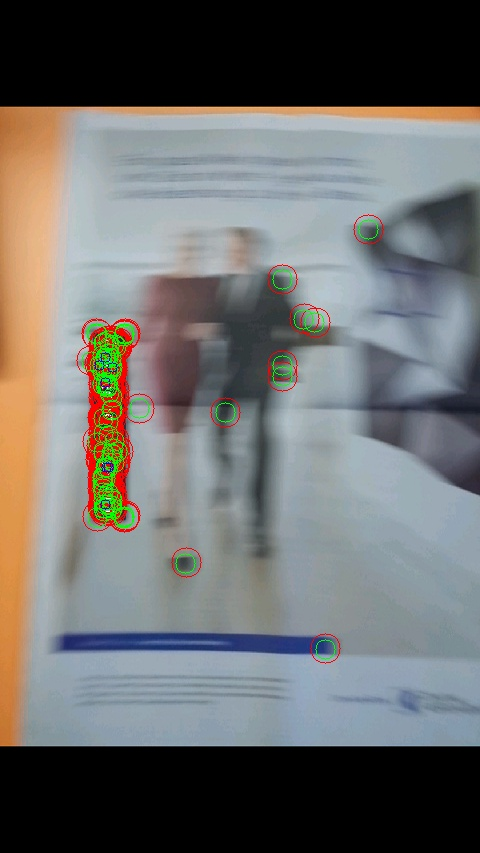
\includegraphics[width=\textwidth]{badly1}
                \caption{keypoint detected in badly blurred image}
                \label{fig:badly1}
        \end{subfigure}
        ~ %add desired spacing between images, e. g. ~, \quad, \qquad etc.
          %(or a blank line to force the subfigure onto a new line)
        \caption{keypoints detectd in different images}\label{fig:images}
\end{figure}

From the table and figures above, we can easily observe the correlation between inputted blurred image and time consuming of homograph computation, which also confirm our guess at beginning. We also observed that blurred image will substantially decrease inlier ratio, which will also cause problem for later processing. In this sense, we should try to avoid motion blur, and use method to decrease the effect when motion blur occur.


\subsection{KLT}

The KLT tracker is a method based on the idea of sparse optical flow. Given a set of initial points it tries to find these points in their vicinity in the subsequent frame. As this is a locally confined method it offers distinct advantages and drawbacks.

\section{Implementation}

\section{Results}

Our results go here


\subsubsection{Equations}

There are three types of equations available: inline equations, for
example $y=mx + c$, which appear in the text, unnumbered equations
$$y=mx + c,$$
which are presented on a line on its own, and numbered equations
\begin{equation}
  \label{eq:linear}
  y = mx + c
\end{equation}
which you can refer to at a later point (Equation~(\ref{eq:linear})).\\

\subsubsection{Tables and Figures}

Tables and figures are ``floating'' objects, which means that the text
can flow around it.
Note
that \texttt{figure*} and \texttt{table*} cause the corresponding
figure or table to span both columns.



\section{Summary}

A short summary of what we have found.

\section*{Acknowledgements}
The author thanks Christian Sigg for his careful reading and helpful
suggestions.

\bibliographystyle{IEEEtran}
\bibliography{nft}
\end{document}
